\documentclass[en]{../../../../../../eplexam}

\usepackage{../../../mmc-MECA1901-exam}

\hypertitle{Mécanique des milieux continus}{5}{MECA}{1901}{2014}{Janvier}
{Vincent Schellekens\and Antoine de Comité\and Aurélien Pignolet\and Mamadou Segpa\and Philippe Greiner}
{Philippe Chatelain et Issam Doghri}

\section{Théorie}

\begin{itemize}
  \item Interpréter le terme $D_{23}$ du tenseur des taux de déformation. Utiliser un dessin pour
votre explication.

\begin{solution}
Rappelons d'abord la définition de $D_{23}$\footnote{$D_{23}$ et $D_{32}$ ont une valeur identique mais ne sont pas équivalents physiquement. En effet, le $1^{er}$ indice correspond à la direction de la normale sortante de la face d'application, tandis que le $2^{eme}$ correspond à la direction de la contrainte.} en coordonnées cartésiennes :

\begin{equation}
D_{23} = D_{32} = \frac{1}{2}(\PDeriv{v_2}{x_3}+\PDeriv{v_3}{x_2})
\end{equation}

Il s'agit du \textit{taux de déformations de cisaillement} associé aux directions $e_2,e_3$ et comporte deux termes, mesurant la variation de la composante en $e_2$ de la vitesse selon $x_3$ et vice versa.

Voir \figuref{def}.
\end{solution}

\begin{figure}[H]
\centering
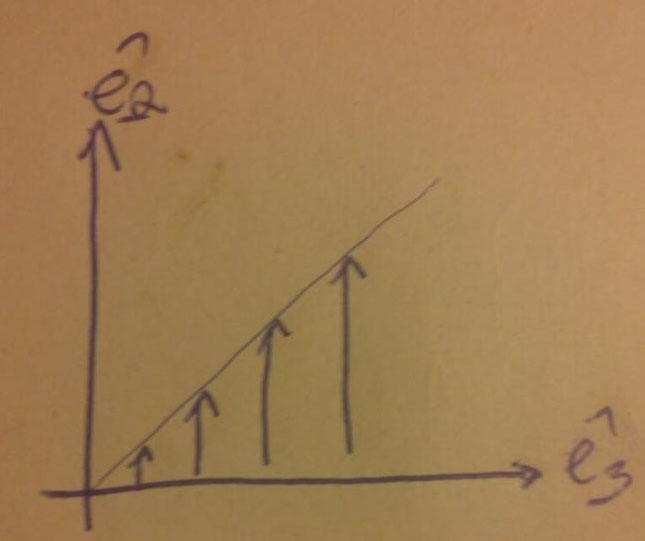
\includegraphics[scale = 0.2]{tauxDefor}
\caption{(Vite fait) si les flèches représentent le champ de vitesse on a ici un tenseur taux de déformations nul sauf pour la composante $D_{23}$ (et $D_{32}$), due au terme $\PDeriv{v_2}{x_3}$ non nul.}
\label{fig:def}
\end{figure}

\item \textbf{Etablir} l'expression du rotationnel d’un champ vectoriel $\mathbf{v}$ en coordonnées-composantes
cylindriques.

\begin{solution}
L'astuce ici est de se rappeler que les vecteurs de base cylindriques varient dans l'espace. Par conséquent, quand on applique un opérateur différentiel spatial, des termes ``supplémentaires'' vont apparaitre. On prend l'expression de l'opérateur nabla en coordonnées cylindriques :

\begin{equation}
\nabla = \Base{r} \PDeriv{}{r} + \Base{\theta}\frac{1}{r}  \PDeriv{}{\theta} + \Base{z} \PDeriv{}{z}
\end{equation}

On calcule ensuite le rotationnel d'un vecteur $\textbf{A}$ en effectuant le produit vectoriel :
\begin{align*}
\nabla \wedge \textbf{A} = (\Base{r} \PDeriv{}{r} + \Base{\theta}\frac{1}{r}  \PDeriv{}{\theta} + \Base{z} \PDeriv{}{z}) \wedge (\Base{r} A_r + \Base{\theta} A_{\theta} + \Base{z} A_z) \\
= \Base{r} \wedge \PDeriv{}{r} (\Base{r} A_r + \Base{\theta} A_{\theta} + \Base{z} A_z) + \Base{\theta}\frac{1}{r} \wedge \PDeriv{}{\theta} (\Base{r} A_r + \Base{\theta} A_{\theta} + \Base{z} A_z) + \Base{z} \wedge \PDeriv{}{z} (\Base{r} A_r + \Base{\theta} A_{\theta} + \Base{z} A_z)
\end{align*}

On rappelle que, pour la dérivée selon theta, il ne faut pas oublier que : $\PDeriv{\Base{r}}{\theta} = \Base{\theta}$ et  $\PDeriv{\Base{\theta}}{\theta} = -\Base{r}$ :

\begin{align*}
\nabla \wedge \textbf{A} = \Base{r} \wedge (\Base{r} \PDeriv{A_r}{r} + \Base{\theta} \PDeriv{A_{\theta}}{r} + \Base{z} \PDeriv{A_z}{r}) \\
+ \Base{\theta}\frac{1}{r} \wedge (\Base{r} \PDeriv{A_r}{\theta} + \Base{\theta} A_r + \Base{\theta} \PDeriv{A_{\theta}}{\theta} - \Base{r} A_{\theta} + \Base{z} \PDeriv{A_z}{\theta}) \\
+ \Base{z} \wedge (\Base{r} \PDeriv{A_r}{z} + \Base{\theta} \PDeriv{A_{\theta}}{z} + \Base{z} \PDeriv{A_z}{z})
\end{align*}

On effectue maintentant le produit vectoriel :

\begin{align}
\nabla \wedge \textbf{A} = 0 + \Base{z} \PDeriv{A_{\theta}}{r} - \Base{\theta} \PDeriv{A_z}{r} \\
+ \frac{1}{r} (-\Base{z} \PDeriv{A_r}{\theta} + 0 + 0 + \Base{z} A_{\theta} + \Base{r} \PDeriv{A_z}{\theta}) \\
+ \Base{\theta} \PDeriv{A_r}{z} - \Base{r} \PDeriv{A_{\theta}}{z} + 0
\end{align}

En réarrangeant les termes, on retrouve bien l'expression du rotationnel en coordonnées cylindriques.
\end{solution}

\item Interprétez les termes du théorème de Reynolds écrit pour un volume matériel $\Omega(t)$,
dans ces deux expressions
\begin{align}
  \frac{D}{D\text{t}}\mathcal{I}(t) & = \int_{\text{$\Omega$}(\text{t})}\left(\frac{D\phi}{D\text{t}}+\phi \nabla \cdot \mathbf{v} \right) \dif v\\
                                    & = \int_{\text{$\Omega$}(\text{t})}\frac{\partial \phi}{\partial \text{t}} \text{dv} +\oint_{\partial \text{$\Omega$}(\text{t})}\phi \mathbf{v} \cdot \hat{\mathbf{n}} \dif s.
\end{align}
Comment passe-t-on de l'une à l'autre?

\begin{solution}
\begin{align*}
\frac{D}{D\text{t}}\mathcal{I}=\int_{\text{$\Omega$}(\text{t})}\left(\frac{D\phi}{D\text{t}}+\phi \nabla \cdot \text{v} \right) \text{dv}\\
\frac{D}{D\text{t}}\mathcal{I}=\int_{\text{$\Omega$}(\text{t})}\frac{\partial \phi}{\partial \text{t}} \text{dv} +\oint_{\partial \text{$\Omega$}(\text{t})}\phi \text{v} \cdot \hat{\text{n}}\text{ds}
\end{align*}

Reprenons la première expression et interprétons la physiquement. Tout d'abord, on peut dire qu'elle est trop mignonne. Le premier terme qu'on retrouve dans la somme correspond à la variation du champ $\phi$ en suivant le point matériel tandis que le second terme correspond lui à la déformation du volume associé à ce même point matériel.

Pour ce qui est la seconde expression, elle peut être interprétée comme la somme de la variation à position fixée et du flux à travers la surface.

Montrons maintenant comment passer de la première expression à la seconde:

\begin{align*}
\frac{D}{D\text{t}}\cal{I} &=\int_{\text{$\Omega$}(\text{t})}\left(\frac{D\phi}{D\text{t}}+\phi \nabla \cdot \bm{v} \right) \text{dv}\\
& = \int_{\text{$\Omega$}(\text{t})}\left(\frac{\partial \phi}{\partial \text{t}}+\bm{v} \cdot \nabla  \phi + \phi \nabla \cdot \bm{v}\right)dv\\
& = \int_{\text{$\Omega$}(\text{t})}\left(\frac{\partial \phi}{\partial \text{t}}+\nabla\cdot (\phi \bm{v})\right)dv\\
& = \int_{\text{$\Omega$}(\text{t})}\frac{\partial \phi}{\partial \text{t}}dv +\oint_{\partial \text{$\Omega$}(t)}\phi \bm{v}\cdot \hat{n}ds
\end{align*}
Pour passer de la première à la seconde ligne, il faut développer la dérivée particulaire. Pour passer de la seconde ligne à la troisième, il faut se souvenir de la définition de dérivée d'un produit et pour passer à la dernière (mais non la moindre\dots) ligne, il faut utiliser le théorème de Green-Ostrogradski.
\end{solution}


\item
Quelle est la plus grande contrainte normale principale dans un tube mince soumis à
une pression interne?

\begin{solution}
La plus grande contrainte est $\sigma_{\theta \theta}$, aussi appelé l'effort circonférentiel. (Voir exemple 4.2.4 du livre.)
On a trois candidats : $\sigma_{rr}$, $\sigma_{\theta \theta}$ et $\sigma_{zz}$. La contrainte $\sigma_{rr}$ est imposée aux surfaces intérieures et extérieures du tube, et vaut $p_i$ à l'intérieur et $p_e$ à l'extérieur ($p_i > p_e$), on peut donc dire que $p_i$ est la valeur maximale de $\sigma_{rr}$. En suivant les calculs détaillés p114 du livre, on trouve qu'en outre $\sigma_{\theta \theta} = \frac{p_iD}{2h} \gg p_i$ et $\sigma_{zz} = \sigma_{\theta \theta}/2$
\end{solution}

\item Donner les 4 idées/hypothèses qui mènent à l’établissement du modèle de fluide visqueux
newtonien. Faire le lien avec l’expression de la loi des contraintes de ce fluide.

\begin{solution}
\mypar{1) Au repos pas d'autres efforts internes que la pression: \\}
On parle ici de la pression hydrostatique - qui correspond à la pression thermodynamique p - et non pas de la pression des examens :) :
\begin{equation*}
\bm{\sigma}=-p \cal{I}
\end{equation*}
On peut donc écrire, pour tout élément de surface
\begin{equation*}
\bm{t}=\bm{\hat{n}}\cdot \bm{\sigma}=-p \bm{\hat{n}}
\end{equation*}
On peut donc exprimer la force de contrainte en fonction de la pression hydrostatique uniquement.

\mypar{2) Efforts visqueux dus aux taux de déformation sont linéaires:\\}
On peut exprimer le tenseur des contraintes comme ceci:
\begin{equation*}
\bm{\sigma}=\cal{F}(\bm{D})-\text{p}\cal{I}
\end{equation*}
Où $\cal{F}(\bm{D})$ représente les efforts visqueux dus aux taux de déformation.

Calculons la série de Taylor de $\tau_{ij}$ sur \textbf{v} autour de 0:
\begin{equation*}
\tau_{ij}=A_{ijk}v_k+B_{ijkl}\frac{\partial v_k}{\partial x_l}+C_{ijklm}\frac{\partial^2 v_k}{\partial x_l \partial x_m}\cdots
\end{equation*}
Si le fluide a un comportement linéaire par rapport aux taux de déformation, on peut supprimer le troisième terme de cette expression et les suivants. Le premier doit s'annuler pour respecter l'objectivité.

\mypar{3) Le matériau a une réponse isotrope:\\}
Ceci signifie que le tenseur $B_{ijkl}$ doit être un tenseur d'ordre 4 isotrope, on peut donc l'exprimer ainsi:
\begin{equation*}
B_{ijkl}=b_1 \delta_{ij}\delta_{kl}+\frac{b_2}{2}(\delta_{ij}\delta_{jl}+\delta_{il}\delta_{jk})+\frac{b_3}{2}(\delta_{ik}\delta_{jl}-\delta_{il}\delta_{jk})
\end{equation*}
Si on réexprime le tenseur de taux de déformation comme un tenseur isotrope d'ordre 4, on obtient
\begin{equation*}
\tau_{ij}=b_1\frac{\partial v_k}{\partial x_k}\delta_{ij}+\frac{b_2}{2}\left(\frac{\partial v_i}{\partial x_j}+\frac{\partial v_j}{\partial x_i}\right) +\frac{b_3}{2}\left(\frac{\partial v_i}{\partial x_j}-\frac{\partial v_j}{\partial x_i}\right)
\end{equation*}
que l'on peut encore réécrire:
\begin{equation*}
\bm{\tau}=\text{$b_1$}(\nabla\cdot \bm{v})\cal{I}+\text{$b_2$}\bm{D}+\text{$b_3$}\bm{\text{$\Omega$}}
\end{equation*}

\mypar{4) La rotation solide ne crée pas de contraintes:\\}
On peut donc écrire le taux de déformation comme ceci:
\begin{equation*}
\bm{\tau}=b_1(\nabla\cdot \bm{v})\cal{I}+\text{$b_2$}\bm{D}
\end{equation*}

On sait que $\bm{\sigma}=\bm{\tau}-p\cal{I}$, et que le taux de déformation peut s'écrire $\bm{\tau}=2\mu \bm{D}+\lambda (\trace\bm{D})\cal{I}$. En utilisant les décompositions sphérique et déviatoire d'un tenseur, on peut écrire successivement:
\begin{align*}
\bm{\tau}=2\mu \left( \bm{D}-\frac{1}{3}(\trace\bm{D})\cal{I}\right)+\left(\frac{2}{3}\mu+\lambda\right)(\trace\bm{D})\cal{I}\\
\bm{\sigma}=2\mu \left( \bm{D}-\frac{1}{3}(\trace\bm{D})\cal{I}\right)+\left(\frac{2}{3}\mu+\lambda\right)(\trace\bm{D})\cal{I}-\text{p} \cal{I}
\end{align*}
\end{solution}
\end{itemize}

\includepdf[pages={3}]{mmc-MECA1901-exam-2014-Janvier-Majeure-Official.pdf}
\ifthenelse{\equal{\Sol}{false}}{}
{\includepdf[pages={4-5}]{mmc-MECA1901-exam-2014-Janvier-Majeure-Official.pdf}}
\includepdf[pages={6}]{mmc-MECA1901-exam-2014-Janvier-Majeure-Official.pdf}
\ifthenelse{\equal{\Sol}{false}}{}
{\includepdf[pages={7-9}]{mmc-MECA1901-exam-2014-Janvier-Majeure-Official.pdf}}

\end{document}
